
Existem diversos \textit{benchmarks} que especificam e simulam cargas de trabalho para avaliarem sistemas computacionais. No entanto, não existe nenhum \textit{benchmark} que possibilite uma avaliação em regime transiente. Este capítulo apresenta e defini uma metodologia de extensão de avaliação em regime transiente para \textit{benchmarks} aproveitando toda a sua maturidade e robustez.


\subsection{\textit{Benchmark} na Computação em Nuvem}
\label{sec-benchmark-web}

\section{A metodologia}
\label{sec-method}

Diversos autores \cite{Hinnant1988, Price1989, KaiSachs2010, Folkerts2013, Marco2012} reconhecem a falta de uma metodologia estabelecida para o desenvolvimento de \textit{benchmarks}. Essa seção, apresenta uma metodologia de extensão para analise transiente através de um \textit{benchmark}. 

A metodologia de extensão descreve as etapas necessárias para as modificações, a seguinte metodologia permite que se obtenha uma carga de trabalho que estimule o sistemas a apresentar a sua dinâmica, assim possibilita a analise transiente do sistema. De acordo com \cite{KaiSachs2010}, uma metodologia de desenvolvimento de \textit{benchmarks} deve incluir o seu processo de desenvolvimento, bem como a sua execução e análise dos seus resultados. 

O objetivo da metodologia é possibilitar que qualquer \textit{benchmark} possa avaliar um sistema em regime transiente afim de descreve a capacidade de resposta e eficiência em reagir às mudanças nas condições de tempo de execução através de modificações feitas no \textit{benchmark}, não tendo a necessidade de desenvolver um; para tanto é fundamental seguir as características presente no \textit{benchmarks}, conforme descrito nessa seção.

De um modo geral, a metodologia de extensão para analise em regime transiente pode ser dividida em três fases:

\begin{enumerate}
	\item Para expor a dinâmica de um sistema é necessário estimulá-lo, a carga de trabalho é quem estimulará o sistema. Logo, a primeira fase é a identificação da implementação do gerador de carga no \textit{benchmark}. Muitas vezes, essa fase é específico para um conjunto de classes, que permite a caracterização da carga de trabalho. 
	Essa implementação é composta por classes ou funções, influenciado diretamente pela linguagem em que o \textit{benchmark} foi desenvolvido, esse conjunto de código é um componente básico do \textit{benchmark} que refere-se a uma unidade de trabalho genérico que envia a carga para o sistema. Alguns \textit{benchmarks} incluem solicitações HTTP, chamadas de procedimento remoto, invocações de serviços Web, transações de banco de dados, comandos interativos ou também mesmo poderia ser composto de múltiplas tarefas de processamento, por exemplo sessões de cliente que compreendem várias solicitações ao sistema, etc.\cite{Kounev2005}
	A escolha dos componentes de carga são definidos em função da natureza dos serviços prestados pelo sistema e sobre os objetivos de modelagem. Uma vez que, em quase todos os casos, esses componentes pode ser considerado como uma espécie de pedidos ou transações processadas pelo sistema, que, muitas vezes, se referem a eles como os pedidos e transações.\cite{Kounev2005}
		
	\begin{figure}[htb]
		\caption{Comportamento de métrica transiente}
		\label{fig:funcoes1}
		\centering
		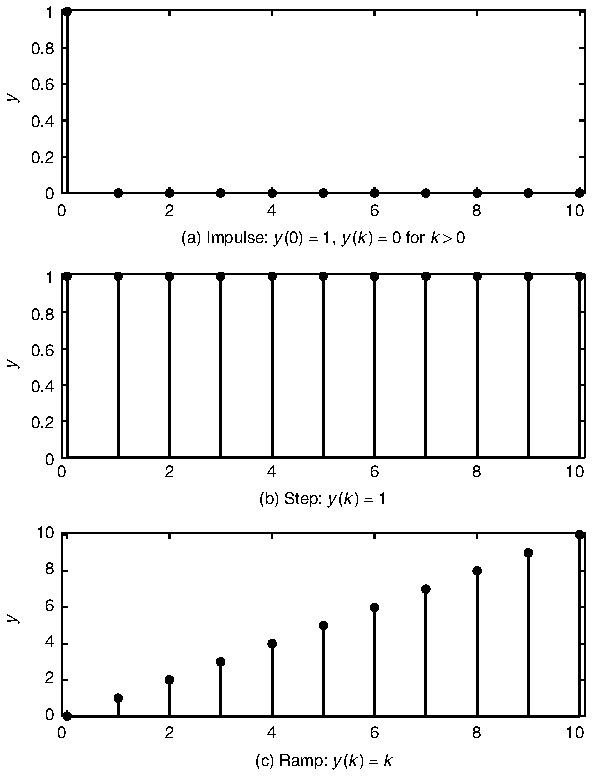
\includegraphics[scale=1]{funcoes1.pdf}
		\fdireta{Hellerstein2004}
	\end{figure}
	
	%\begin{figure}
	%	\begin{center}
	%		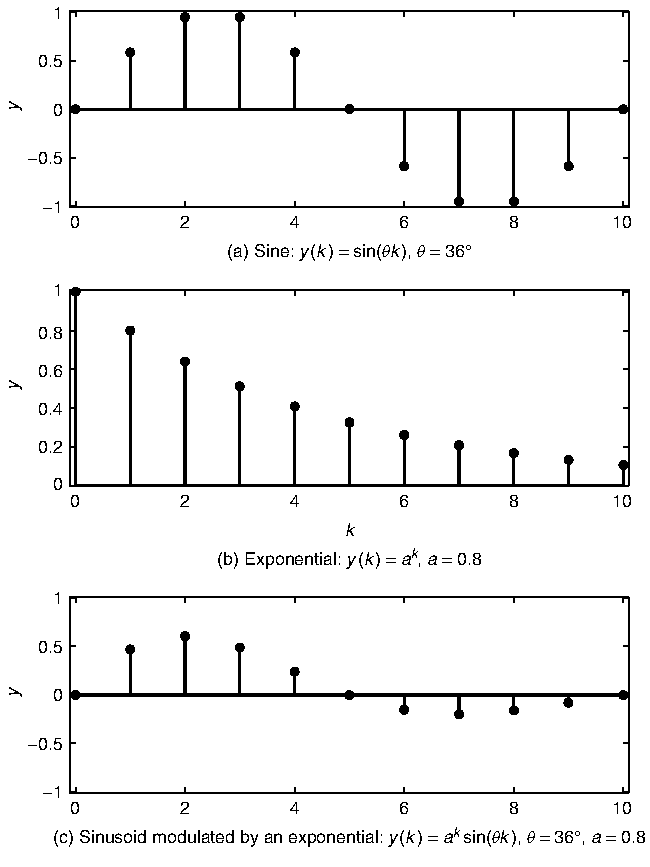
\includegraphics[width=0.8\textwidth]{img/funcoes2.pdf}
	%		\caption{Sinais em tempo discreto comuns, parte 2. \cite{Hellerstein2004}}
	%		\label{fig:funcoes2}
	%	\end{center}
	%\end{figure} 
	
	Segundo \cite{Nobile2013} uma alteração na entrada (carga de trabalho) fará com que o sistema saia do estado em regime estacionário e entre em um período de regime transiente e para descrever a dinâmica de um sistema, comumente, o ganho em regime estacionário é calculado para uma entrada degrau unitário. \textit{Para realizar a analise transitória do sistema, é preciso utilizar cargas de trabalho que possam provocar comportamentos propícios}, onde as caraterísticas dinâmicas do sistema sejam claramente observadas, em \cite{Hellerstein2004}, são propostas algumas funções, ou sinais, de perturbação, por exemplo: impulso, degrau, rampa, seno, exponencial, seno modulada por uma exponencial, etc.  Essas funções são apresentadas na figura \ref{fig:funcoes1}.% e \ref{fig:funcoes2}.
	
	Assim as modificações devem ser feitas no \textit{engine} do gerador de carga do \textit{benchmark}, pois nele que se encontra o componente que tem o conjunto de parâmetros que caracterizam a carga de trabalho. A carga de trabalho resultante deve expressar ao menos uma das funções apresentadas.
		
	
	\item O segundo passa da metodologia, é medir o comportamento do sistema com a ajuda de métricas. A métrica é uma função que transforma resultados medidos em uma forma que seja facilmente compreendida. \cite{Folkerts2013} As métricas de referência deve permitir caracterizar e quantificar o comportamento do sistema quando enfrenta perturbações (ou seja, falhas, ataques, e variações de ambiente operacional).\cite{Marco2012} As métricas tradicionais, de analise estacionaria, não pode capturar o comportamento transitório do sistema em resposta às variações de carga implementada no primeiro passo da metodologia.
	
	No contexto de avaliação transiente, \cite{Rosu1997} afirma que a reatividade da métrica é muitas vezes mais importante do que a otimização da mesma, no mesmo trabalho, \cite{Rosu1997} apresenta a característica e comportamento de uma métrica transiente, conforme ilustrado pela figura \ref{fig:transient-metric}, que são: 
	\begin{itemize}
		\item \textbf{\textit{Reaction Time} (Tempo de reação)} - o período entre a ocorrência da variação crítica e a conclusão da promulgação realocação de correção;
		
		\item \textbf{\textit{Recovery Time} (Tempo de Recuperação)}  - o intervalo entre a conclusão promulgação e da restauração de um nível de desempenho aceitável;
		
		\item \textbf{\textit{Performance Laxity} (Frouxidão performance)} - a diferença entre o required v performance, e o desempenho em estado estacionário, após a redistribuição;
	\end{itemize}
	
	
	\begin{figure}[htb]
		\caption{Comportamento de métrica transiente}
		\label{fig:transient-metric}
		\centering
		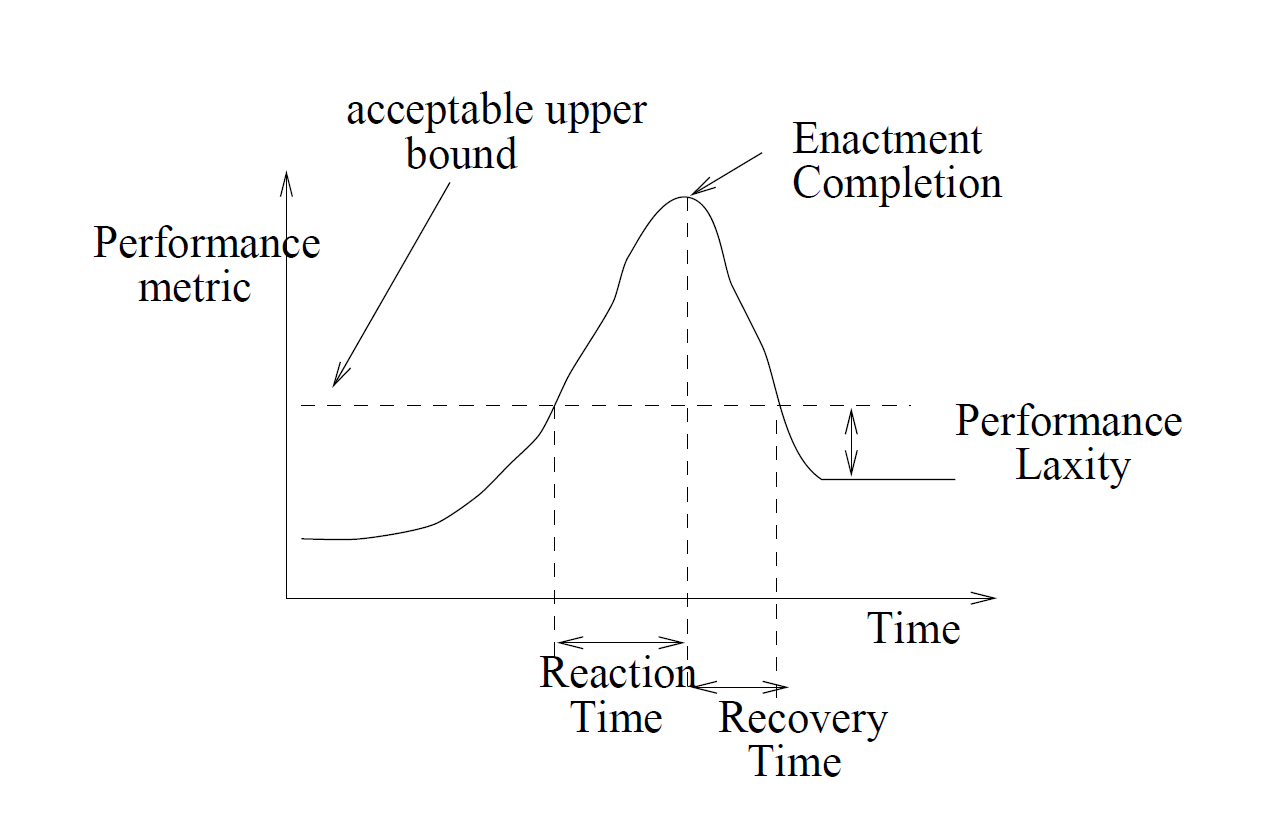
\includegraphics[scale=0.4]{transient-metric.png}
		\fdireta{Rosu1997}		
	\end{figure}
	
	
	A métrica em questão deve ser identifica dentro da realidade e necessidade em que se encontra o sistemas a ser avaliado. Logo será de uma ingenuidade fixar uma métrica para um sistema desconhecido, o importante é que ela tenha o comportamento e as caracteriais apresentadas anteriormente nesse passo da metodologia de extensão. Existem diversos trabalhos dedicados que identificam métricas transiente em vários contextos como o \cite{Binnig2009, Lu2000, Rosu1997}.
	
	\item A última atividade dentro da metodologia de extensão do \textit{benchmark} é a análise e apresentação de resultados. Aqui, os dados bruto de desempenho são obtidos estatisticamente processadas e interpretadas. Para a análise, a metodologia deve fornecer orientações para uma avaliação estatística rigorosa e validação dos dados coletados. Além disso, ele deve fornecer orientações para a apresentação dos resultados estatísticos, os intervalos de confiança presentes em adição à média. Para garantir a replicabilidade, deve, adicionalmente, fornecer diretrizes para a descrição das experiências de \textit{benchmark} realizados.		
	
\end{enumerate}




